\documentclass{article}
\usepackage{blindtext}
\usepackage{graphicx}
\usepackage{hyperref}
\usepackage{listings}
\usepackage[dvipsnames]{xcolor}
\graphicspath{ {./img/} }

\definecolor{vsBlue}{RGB}{31, 90, 179}
\definecolor{kw}{rgb}{0.627,0.126,0.941}
\definecolor{vsFunc}{RGB}{220, 220, 146}
\definecolor{vsBlack}{RGB}{30, 30, 30}
\definecolor{vsClass}{RGB}{78, 201, 151}

\lstset{
    language=C,
    basicstyle=\color{white}\footnotesize\ttfamily,
    %aboveskip={1.0\baselineskip},
    %belowskip={1.0\baselineskip},
    columns=fixed,
    extendedchars=true,
    breaklines=true,
    tabsize=4,
    %prebreak=\raisebox{0ex}[0ex][0ex]{\ensuremath{\hookleftarrow}},
    frame=lines,
    xleftmargin=0ex,
    rulecolor=\color{white},
    showtabs=false,
    showspaces=false,
    showstringspaces=false,
    keywordstyle=\color{vsBlue},
    commentstyle=\color[rgb]{0.133,0.545,0.133},
    stringstyle=\color[RGB]{214, 157, 133},
    numbers=left,
    numberstyle=\small,
    stepnumber=1,
    numbersep=10pt,
    captionpos=t,
    escapeinside={\%*}{*)},
    backgroundcolor=\color{vsBlack}
}

\lstset{emph = {bool, true, false}, emphstyle={\color{kw}}}
\lstset{emph = {printf, scanf, fopen, fclose, fwrite, fread}, emphstyle={\color{vsFunc}}}

\title{Analizzatore analogico}
\author{Antonio Sgalla}
\date{24/05/2023}

\begin{document}

\maketitle

\section{Descrizione del progetto}
Realizzare un campionatore di un segnale analogico a \textbf{8 bit}, alla massima velocità consentita dal processore, che visualizzi graficamente i valori letti su una matrice di led \textbf{8x8} tramite interfaccia \textbf{SPI MAX7219}.
\newline\newline
Il sistema deve consentire di impostare la base dei tempi e quindi visualizzare, per ogni colonna di led, il valor medio progressivo dei valori acquisiti in ingresso.

\section{Funzionamento}
Appena acceso, il prototipo si trova nella modalità di inserimento base dei tempi: tramite il potenziometro di destra è possibile specificare quanti campioni vengono presi per fare la media progressiva, velocizzando o rallentando la visualizzazione a schermo.
Quando si gira questo potenziometro, la matrice illumina più o meno colonne delle due righe centrali, più led vengono illuminati e più l'analisi sarà lenta.
\newline\newline
Premendo il pulsante è possibile passare alla modalità di analisi, contrassegnata dall'illuminazione del led color ciano: bisogna usare il potenziometro di sinistra come input analogico e automaticamente verrà visualizzata la media progressiva dei campioni nella matrice led, rispettando la base dei tempi precedentemente impostata.
In questa modalità i valori verranno visualizzati sulle colonne: ogni colonna corrisponde a una media progressiva di X campioni (variabile sulla base dei tempi).
\newline\newline
Premendo nuovamente il pulsante si torna alla modalità di default, ovvero quella di impostazione della base dei tempi

\section{Schema del circuito}
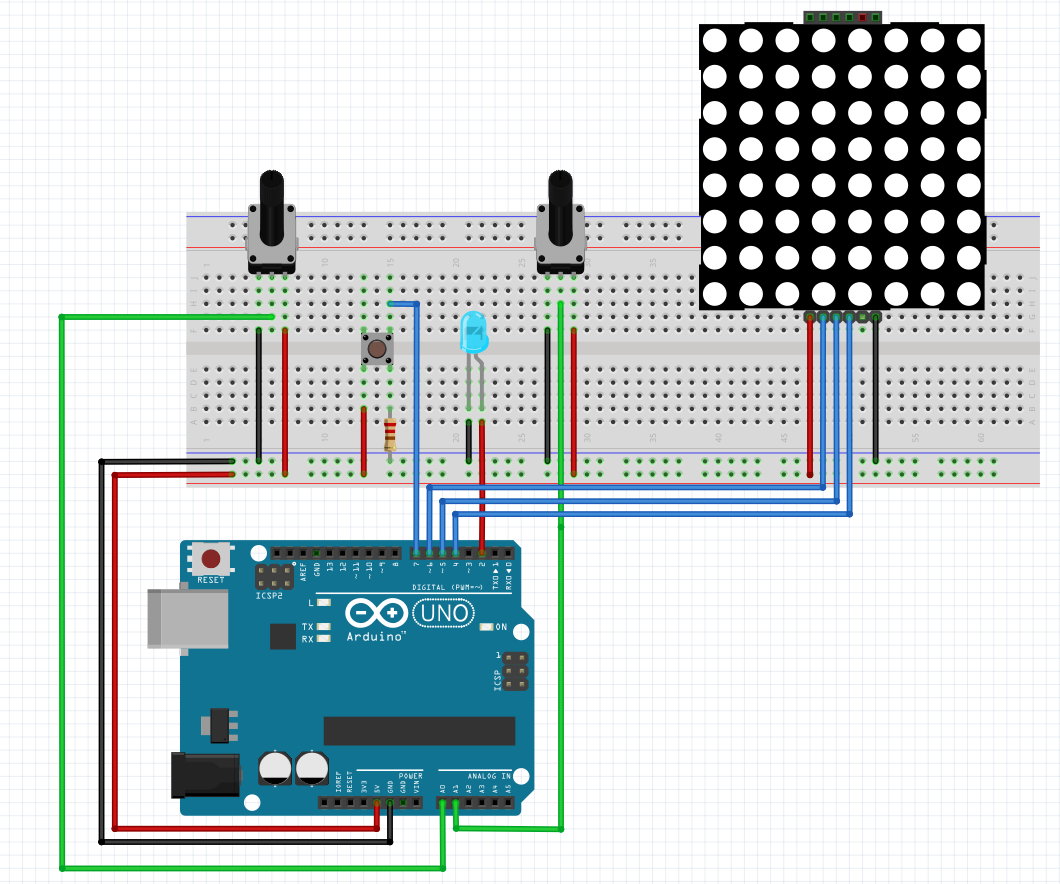
\includegraphics[scale=.4]{progettoFritzing.png}

\section{Diagramma degli stati}
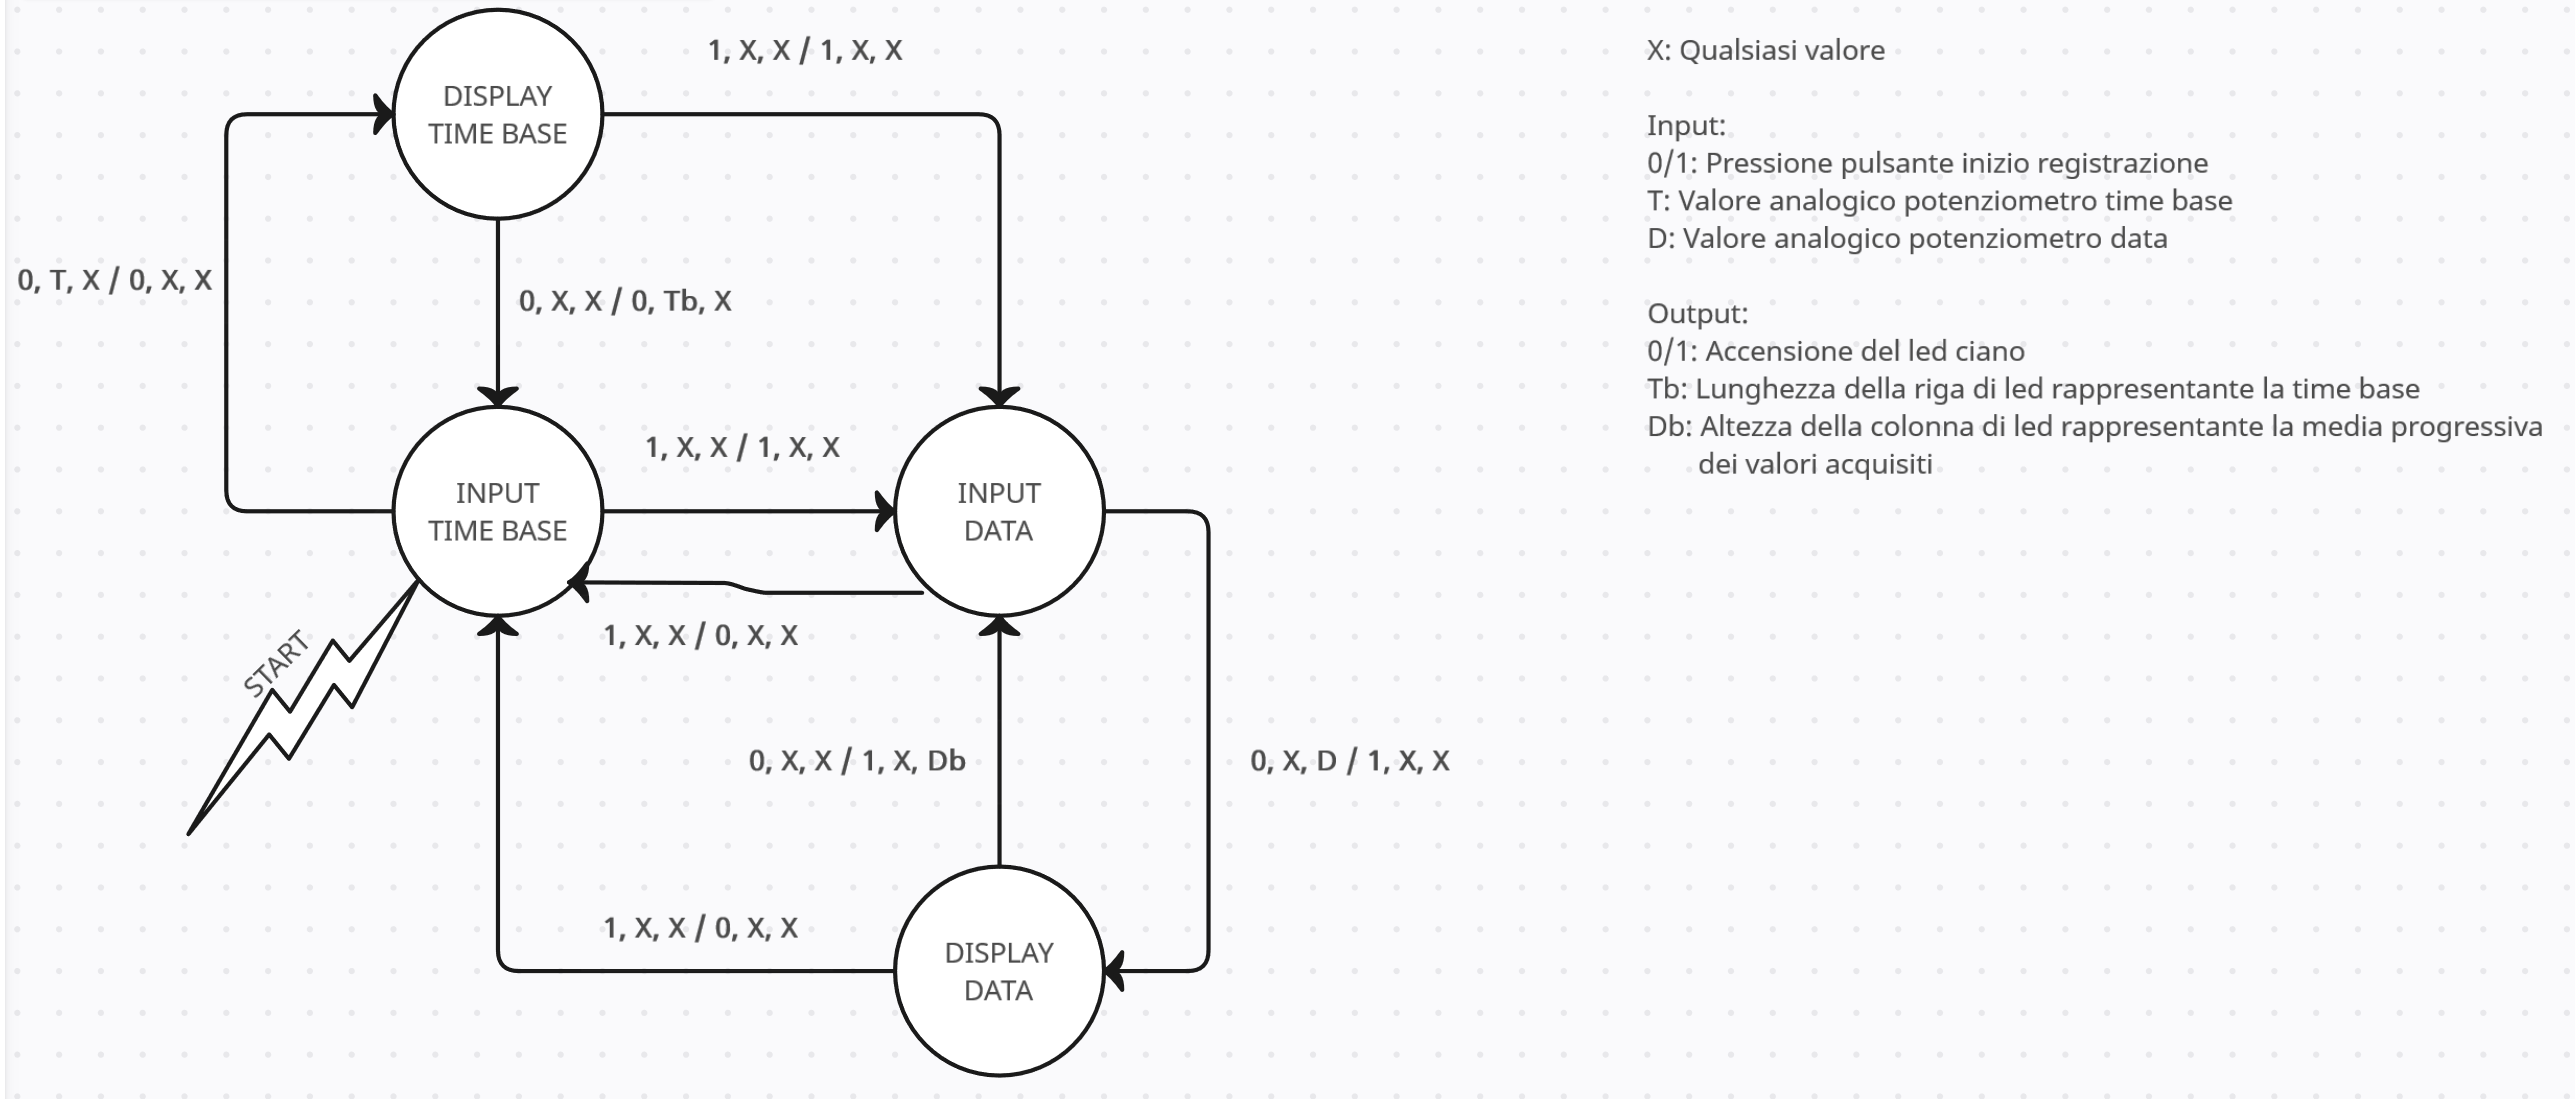
\includegraphics[scale=.2]{diagrammaStati.png}

\section{Flowchart generico}
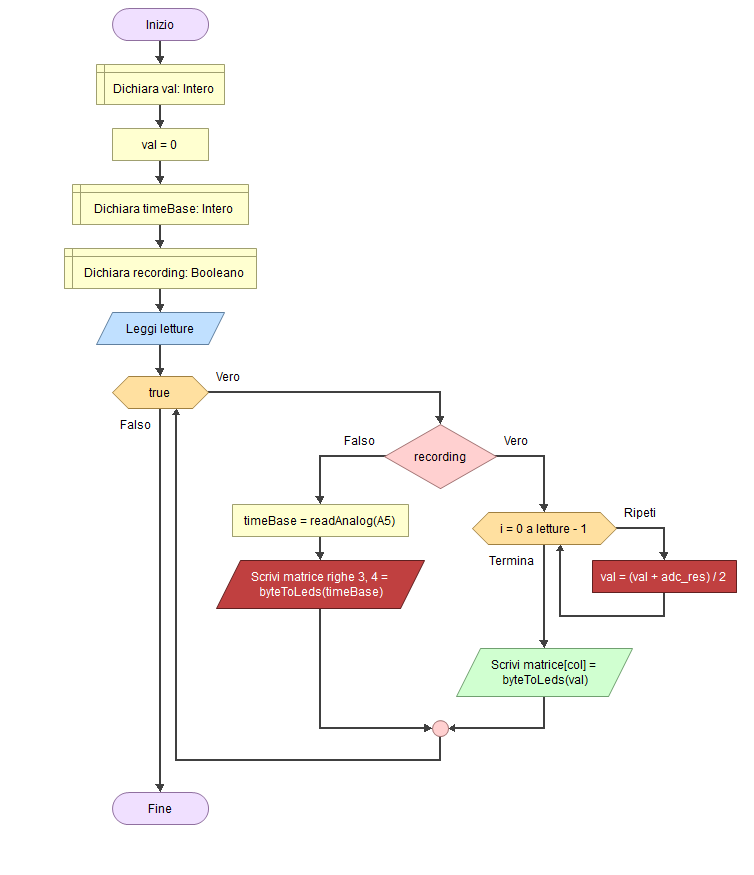
\includegraphics[scale=.4]{genericFlowchart.png}
Questo flowchart è stato fatto all'inizio del progetto, per dargli una direzione.
Non è per nulla dettagliato, serve solo come sketch.

\section{Flowchart specifico}
Includerò solamente le funzioni principali, per le altre è possibile consultare il file \textbf{.fprg} allegato

\subsection{Funzione setup}
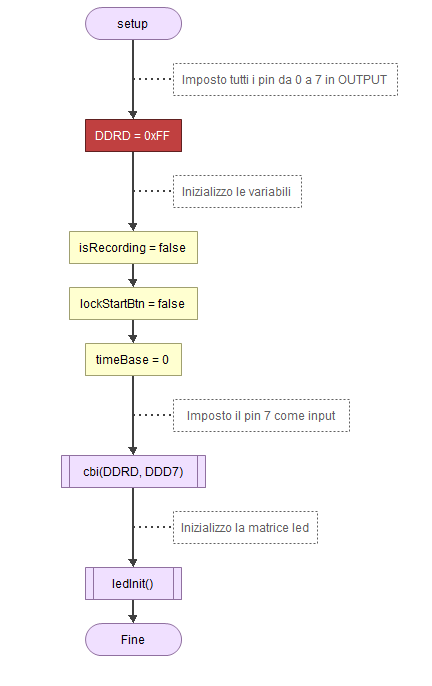
\includegraphics[scale=.60]{funSetup.png}
\subsection{Funzione loop}
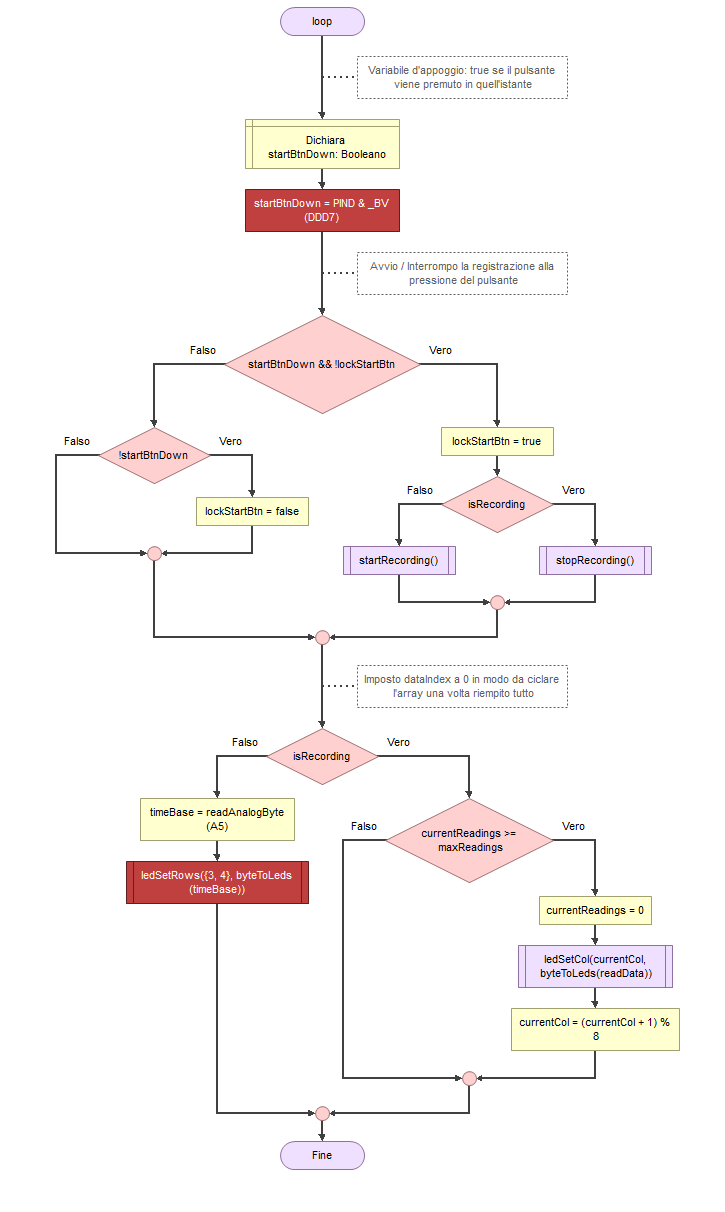
\includegraphics[scale=.50]{funLoop.png}
\subsection{Funzione startRecording}
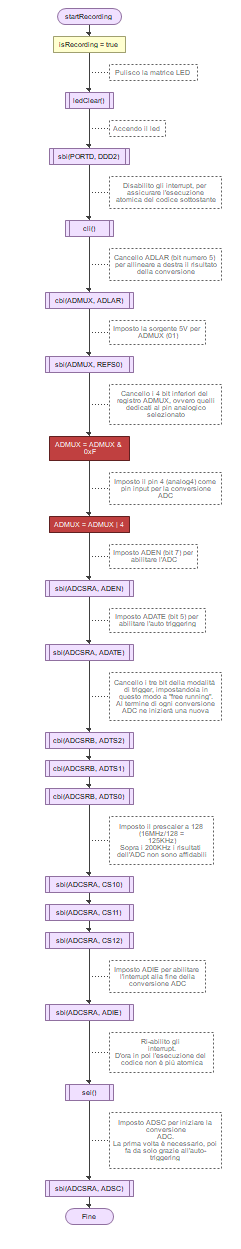
\includegraphics[scale=.50]{funStartRec.png}
\subsection{Funzione stopRecording}
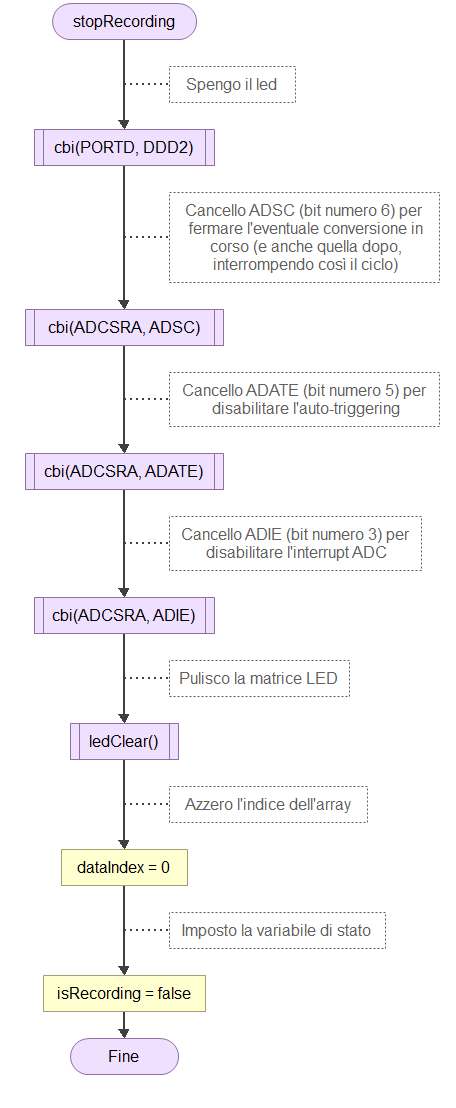
\includegraphics[scale=.60]{funStopRec.png}
\subsection{Funzione di gestione interrupt ADC}
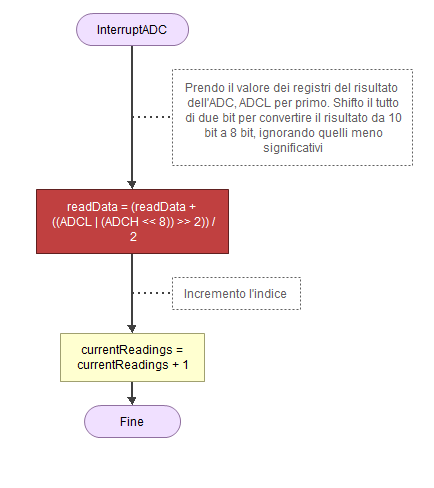
\includegraphics[scale=.60]{funAdcInterrupt.png}
\newpage

\section{Codice arduino}
Includerò solamente le funzioni principali, per le altre è possibile consultare il file \textbf{.ino} allegato

\subsection{Definizione delle macro}
\begin{lstlisting}[]
#define _NBV ~_BV

#define sbi(reg, bit) (reg |= _BV(bit))
#define cbi(reg, bit) (reg &= _NBV(bit))

#define cli() __asm__ __volatile__ ("cli");
#define sei() __asm__ __volatile__ ("sei");
\end{lstlisting}
\newpage

\subsection{Funzione setup}
\begin{lstlisting}[]
void setup() {
    // Imposto tutti i pin da 0 a 7 in OUTPUT
    DDRD = 0xFF;
    
    // Inizializzo la variabile di stato
    isRecording = false;
    
    // Inizializzo la variabile per il meccanismo SET-RESET del pulsante
    lockStartBtn = false;
    
    // Inizializzo la base dei tempi a 0
    timeBase = 0;
    
    // Imposto solamente il pin 7 (bottone) come input
    cbi(DDRD, DDD7);
    
    // Inizializzo la matrice led
    ledInit();
}
\end{lstlisting}
\newpage

\subsection{Funzione loop}
\begin{lstlisting}[]
void loop() {
    // Variabile d'appoggio: true se il pulsante viene premuto in quell'istante
    bool startBtnDown = PIND & _BV(DDD7);
    
    // Meccanismo SET-RESET per chiamare solo una volta la funzione anche se il pulsante viene tenuto premuto
    if (startBtnDown && !lockStartBtn) {
        // SET
        lockStartBtn = true;
        
        if (isRecording) {
        // Fermo la registrazione dei dati
        stopRecording();
        } else {
        // Inizio della registrazione dei dati
        startRecording();
        }
    } else if (!startBtnDown) {
        // RESET
        lockStartBtn = false;
    }
    
    if (isRecording) {
        if (currentReadings >= maxReadings) {
        currentReadings = 0;
        ledSetCol(currentCol, byteToLeds(readData));
        currentCol = (currentCol + 1) % 8;
        }
    } else {
        timeBase = readAnalogByte(A5);
        byte row = byteToLeds(timeBase);
        ledSetRow(3, row);
        ledSetRow(4, row);
    }
}
\end{lstlisting}

\subsection{Funzione gestione interrupt ADC}
\begin{lstlisting}[]
// Interrupt service routine per il completamnto della conversione ADC
ISR(ADC_vect){
  // Cicli di clock: ~67
  
  // Bisogna leggere ADCL per primo
  readData = (readData + (ADCL | (ADCH << 8)) >> 2) / 2;
  currentReadings++;
}
\end{lstlisting}

Per sapere quasi esattamente i cicli di clock necessari per l'esecuzione della funzione sopra riportata, ho disassemblato il programma compilato, ed ho sommato il duty cycle di ogni operazione eseguita, a livello di assembly avr.
\newpage

\begin{lstlisting}[title=Disassembly della funzione]
00000530 <__vector_21>:
530:   1f 92           push    r1
532:   0f 92           push    r0
534:   0f b6           in      r0, 0x3f        ; 63
536:   0f 92           push    r0
538:   11 24           eor     r1, r1
53a:   2f 93           push    r18
53c:   3f 93           push    r19
53e:   8f 93           push    r24
540:   9f 93           push    r25
542:   20 91 78 00     lds     r18, 0x0078     ; 0x800078 <__DATA_REGION_ORIGIN__+0x18>
546:   80 91 79 00     lds     r24, 0x0079     ; 0x800079 <__DATA_REGION_ORIGIN__+0x19>
54a:   38 2f           mov     r19, r24
54c:   35 95           asr     r19
54e:   27 95           ror     r18
550:   35 95           asr     r19
552:   27 95           ror     r18
554:   80 91 f0 01     lds     r24, 0x01F0     ; 0x8001f0 <readData>
558:   82 0f           add     r24, r18
55a:   93 2f           mov     r25, r19
55c:   91 1d           adc     r25, r1
55e:   97 fd           sbrc    r25, 7
560:   01 96           adiw    r24, 0x01       ; 1
562:   95 95           asr     r25
564:   87 95           ror     r24
566:   80 93 f0 01     sts     0x01F0, r24     ; 0x8001f0 <readData>
56a:   80 91 f4 01     lds     r24, 0x01F4     ; 0x8001f4 <currentReadings>
56e:   90 91 f5 01     lds     r25, 0x01F5     ; 0x8001f5 <currentReadings+0x1>
572:   01 96           adiw    r24, 0x01       ; 1
574:   90 93 f5 01     sts     0x01F5, r25     ; 0x8001f5 <currentReadings+0x1>
578:   80 93 f4 01     sts     0x01F4, r24     ; 0x8001f4 <currentReadings>
57c:   9f 91           pop     r25
57e:   8f 91           pop     r24
580:   3f 91           pop     r19
582:   2f 91           pop     r18
584:   0f 90           pop     r0
586:   0f be           out     0x3f, r0        ; 63
588:   0f 90           pop     r0
58a:   1f 90           pop     r1
58c:   18 95           reti
\end{lstlisting}
\newpage

\section{Fotografie progetto fisico}
\subsection{Prototipo spento}
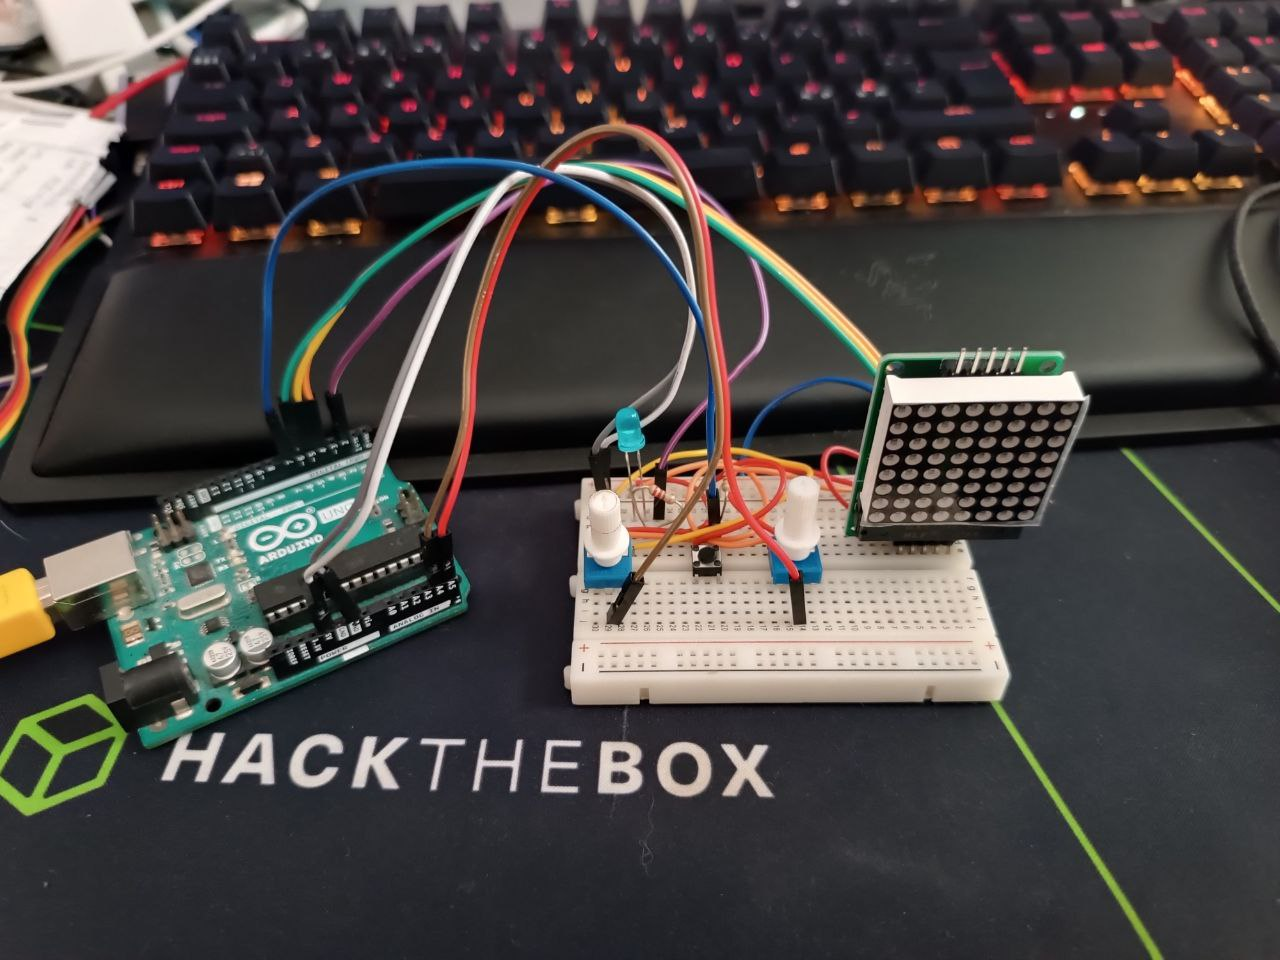
\includegraphics[scale=.25]{protOff.jpg}
\subsection{Prototipo acceso, in modalità inserimento base tempi}
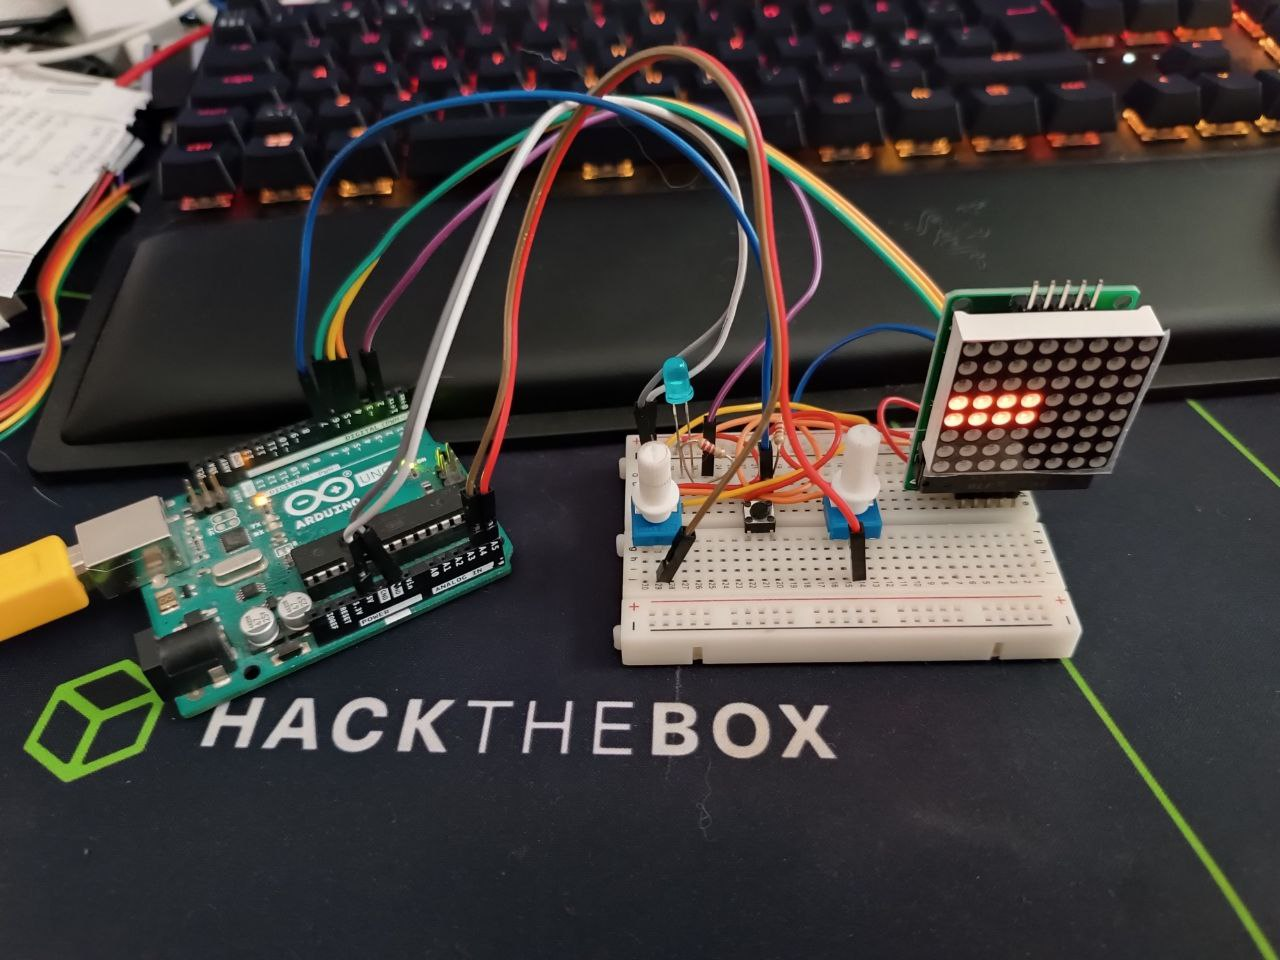
\includegraphics[scale=.25]{protOnIdle.jpg}
\subsection{Prototipo acceso, in modalità analisi}
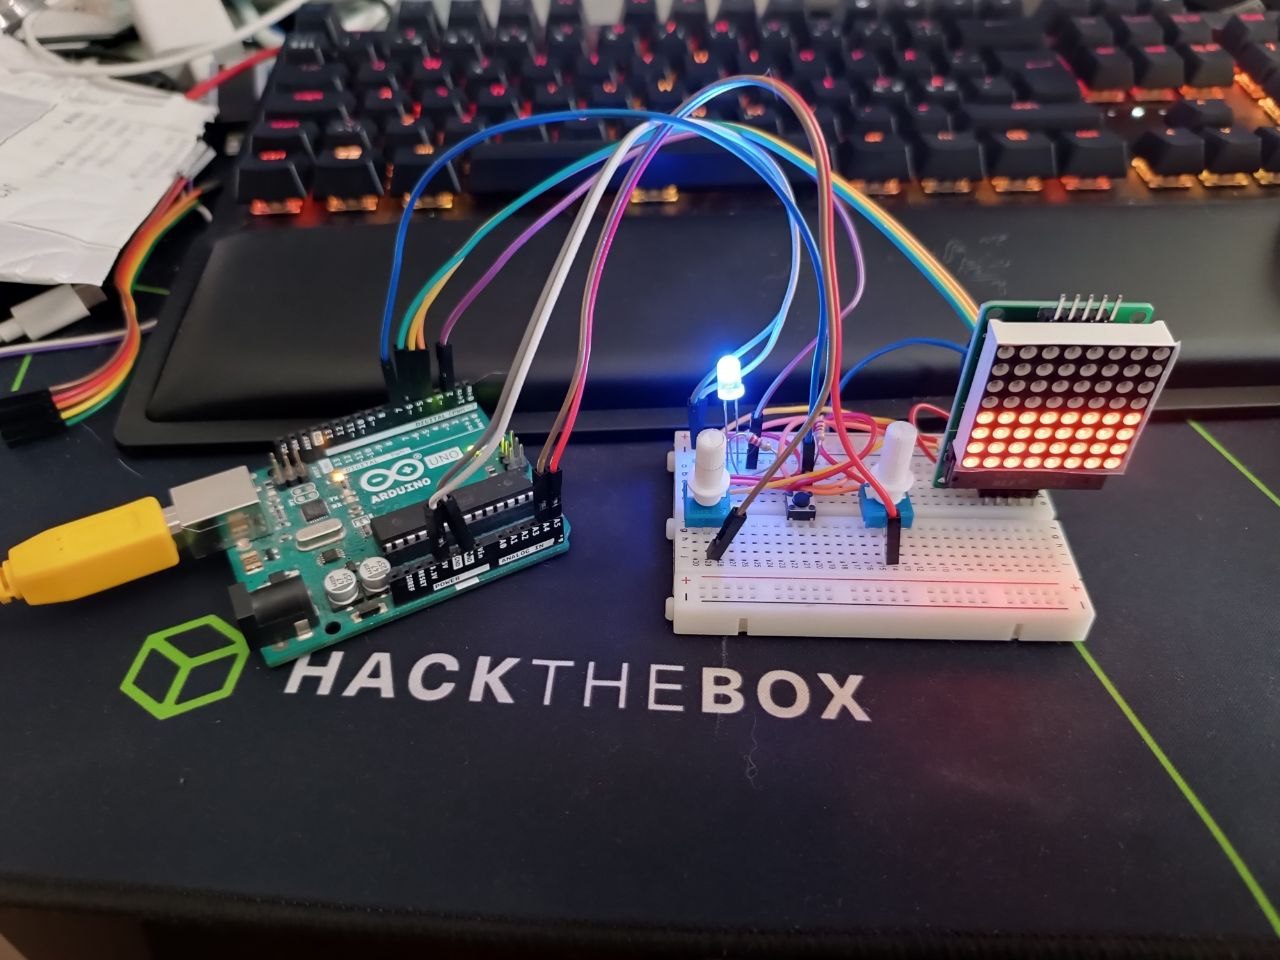
\includegraphics[scale=.25]{protOnRec.jpg}

\section{Webliografia}
\begin{itemize}
    \item \href{https://ww1.microchip.com/downloads/en/DeviceDoc/Atmel-7810-Automotive-Microcontrollers-ATmega328P_Datasheet.pdf}{Datasheet ATmega328P}
    \item \href{https://www.farnell.com/datasheets/29075.pdf}{Datasheet MAX7219 (spunto per comunicazione SPI)}
\end{itemize}

\end{document}